\chapter{OPIS TECHNICZNY}
\label{chapter:opis_techniczny}


\section{Aplikacja wit.ai}
W ramach projektu została stworzona aplikacja w systemie \textit{wit.ai}. Wit.ai to platforma do tworzenia interfejsów interaktywnych, która pozwala na budowanie aplikacji, które rozumieją naturalny język. Wit.ai pozwala na tworzenie modeli językowych, które są w stanie rozpoznawać intencje użytkownika na podstawie zdefiniowanych przez programistę fraz. Aplikacja ta jest wykorzystywana w projekcie do rozpoznawania intencji użytkownika na podstawie zdefiniowanych przez programistę fraz.

\subsection{Intencje i encje}

W celu nauczenia modelu językowego aplikacji wit.ai, należy zdefiniować intencje (ang. \textit{intents}), które mają być rozpoznawane przez aplikację. Intencje to frazy, które użytkownik może napisać, a które mają być zrozumiane przez aplikację. Każda intencja może zawierać wiele przykładów fraz, które są z nią związane. Przykładowe intencje, które zostały zdefiniowane w aplikacji wit.ai to:
\begin{itemize}
    \item \textit{add\_product\_to\_cart} - intencja dodania produktu do koszyka,
    \item \textit{remove\_product\_from\_cart} - intencja usunięcia produktu z koszyka,
    \item \textit{check\_cart} - intencja sprawdzenia zawartości koszyka,
    \item \textit{check\_item\_prices} - intencja sprawdzenia cen produktów,
    \item \textit{check\_item\_price\_in\_store} - intencja sprawdzenia ceny produktu w sklepie
\end{itemize}

Poza intencjami, w aplikacji wit.ai definiuje się również encje (ang. \textit{entities}). Encje to frazy, które mają być rozpoznawane przez aplikację jako konkretne wartości. Encje pomagają również w wykryciu intencji użytkownika. Przykładowe encje, które zostały zdefiniowane w aplikacji wit.ai to:
\begin{itemize}
    \item \textit{product} - encja reprezentująca nazwę produktu,
    \item \textit{store} - encja reprezentująca nazwę sklepu,
    \item \textit{view} - encja reprezentująca widok w aplikacji,
    \item \textit{category} - encja reprezentująca nazwę kategorii produktów
\end{itemize}

Po zdefiniowaniu intencji i encji, aplikacja wit.ai pozwala na trenowanie modelu językowego. Trenowanie modelu polega na przesłaniu do aplikacji wit.ai przykładów fraz, które mają być rozpoznawane przez aplikację. Po przesłaniu przykładów, aplikacja wit.ai trenuje model językowy. Po wstępnym treningu, aplikacja stara się sama sugerować intencje w procesie trenowania modelu. Pozwala to na sprawdzanie w czasie rzeczywistym, czy model językowy poprawnie rozpoznaje encje i intencje. Przykładowe frazy wykorzystane w procesie trenowania modelu to:
\begin{itemize}
    \item \textit{Where to buy apples}
    \item \textit{Remove cheese from cart},
    \item \textit{My app is stuck on loading},
    \item \textit{Is there dairy in castorama?}
\end{itemize}

\subsection{Kreator}

Wytrenowany model należy zaprogramować. W tym celu wit.ai udostępnia kreator (ang. \textit{composer}), który pozwala na zdefiniowanie akcji, które mają być wykonywane po rozpoznaniu intencji przez aplikację. Przykładowe akcje, które zostały zdefiniowane w aplikacji wit.ai przedstawiono na rysunku \ref{fig:wit_ai_composer}.

\begin{figure}[H]
    \centering
    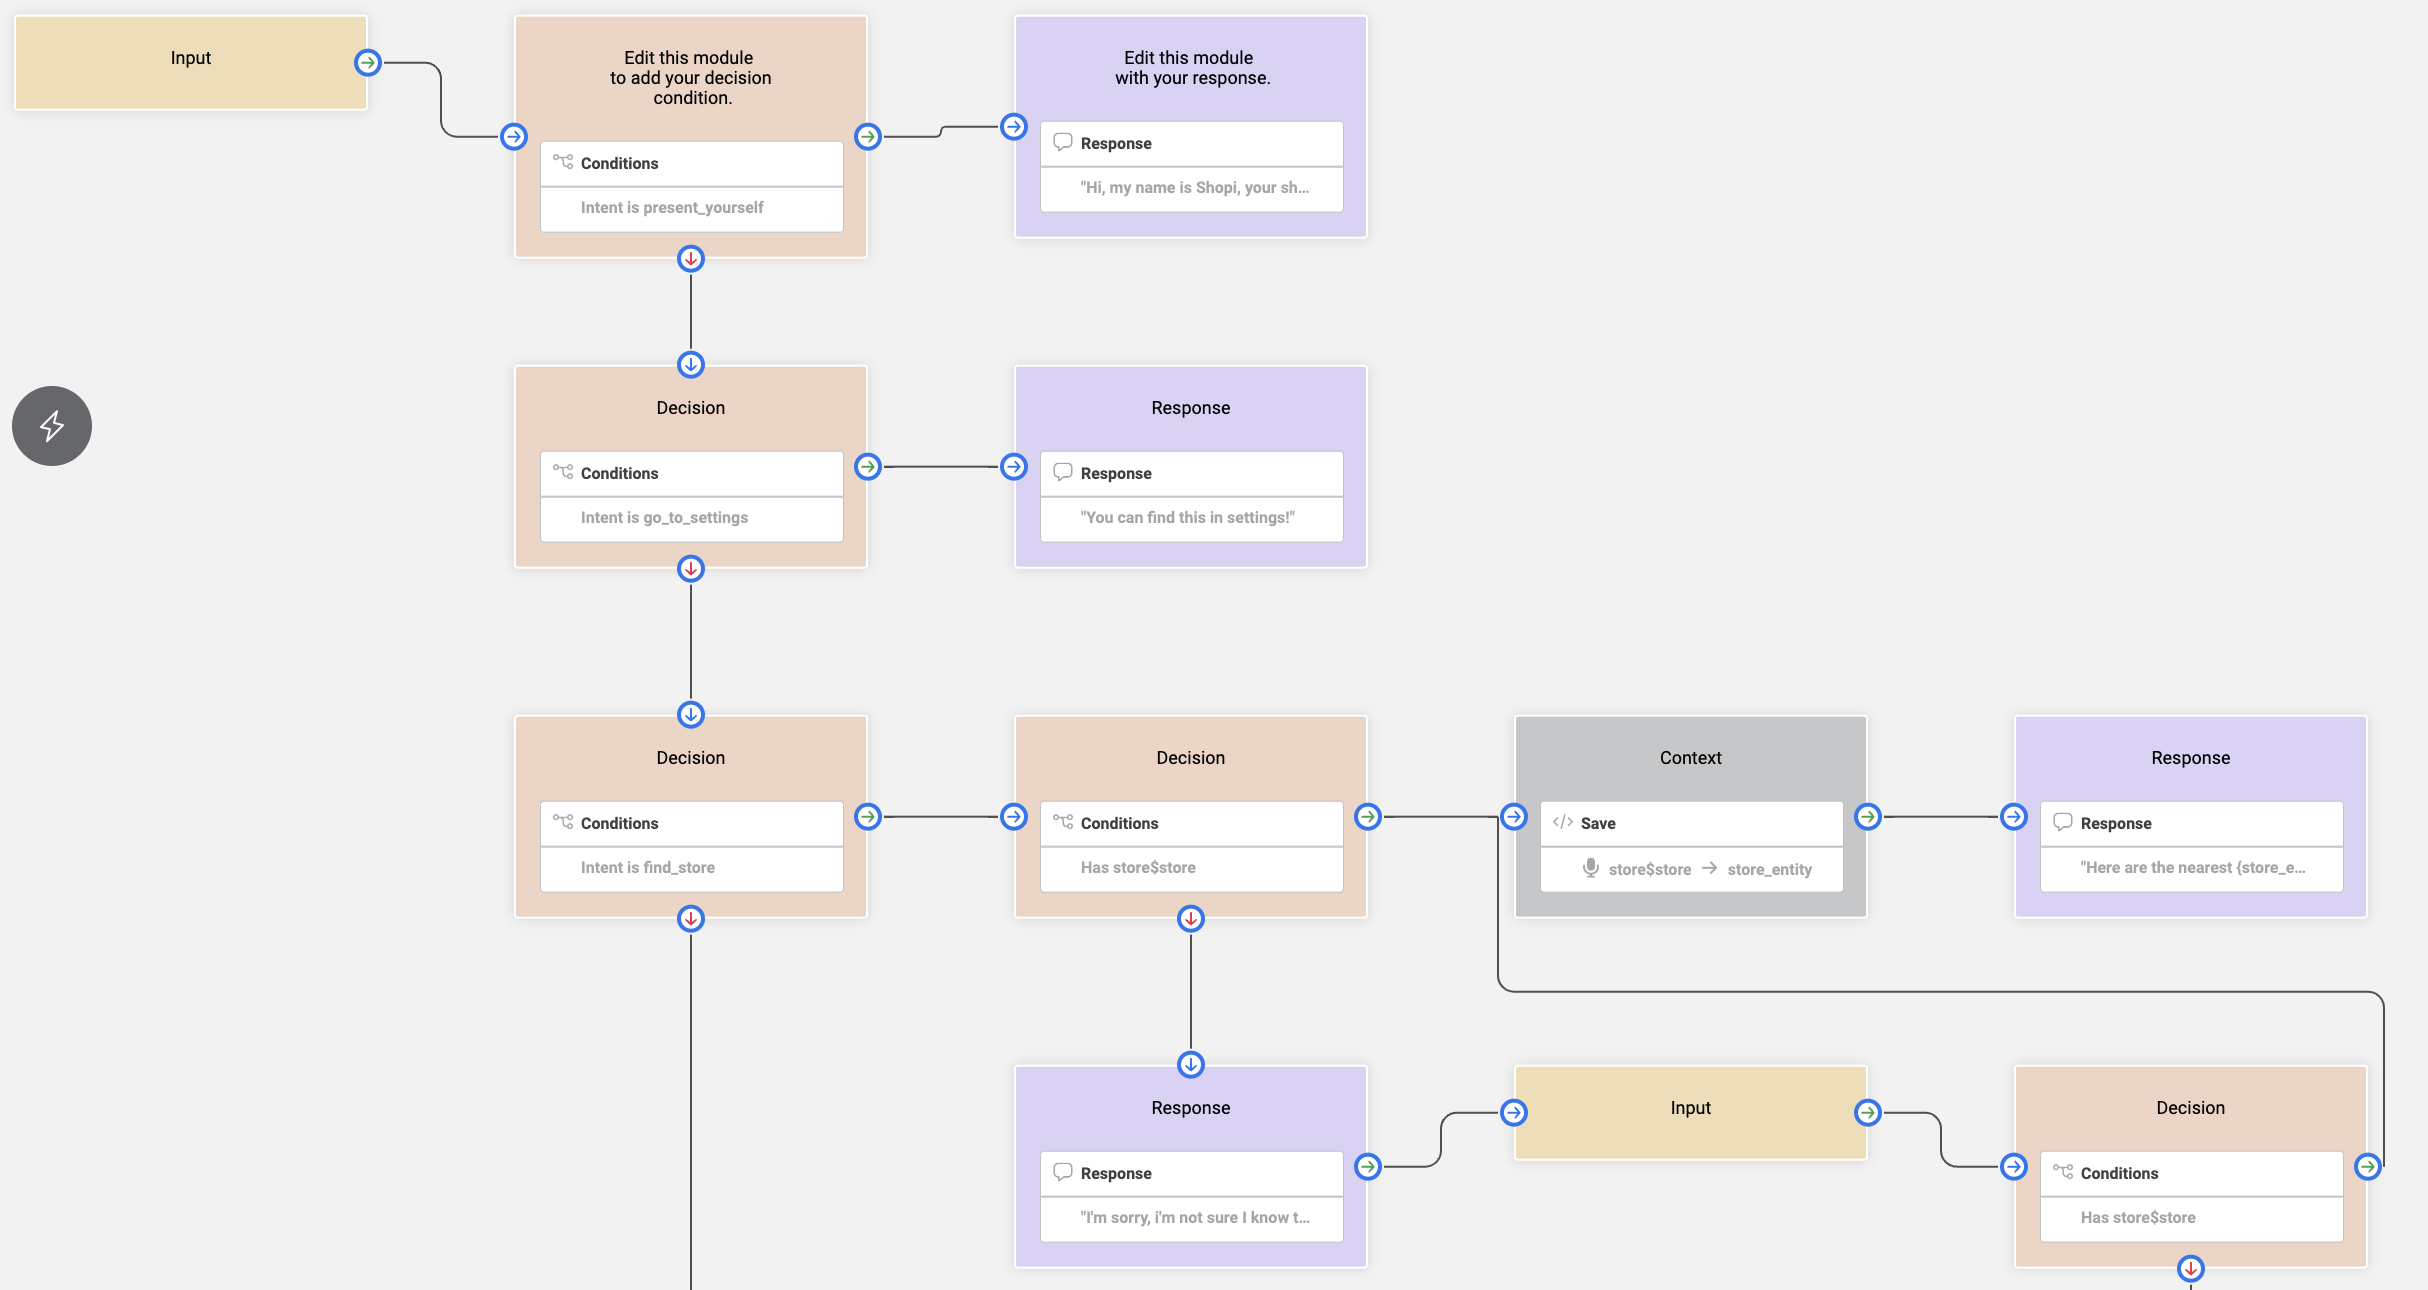
\includegraphics[width=0.8\textwidth]{images/witai_composer.png}
    \caption{Kreator aplikacji wit.ai}
    \label{fig:wit_ai_composer}
\end{figure}

\subsubsection{Akcje}

W ramach kreatora dostępne są 4 moduły blokowe definiujące akcje. Są to:
\begin{itemize}
    \item \textit{Decision} - moduł decydujący o dalszym przebiegu akcji,
    \item \textit{Context} - moduł przechowujący kontekst akcji,
    \item \textit{Input} - moduł pobierający dane wejściowe,
    \item \textit{Response} - moduł generujący odpowiedź.
\end{itemize}

\subsubsection{Decision}

Moduł \textit{Decision} pozwala na zdefiniowanie warunków, które muszą być spełnione, aby akcja mogła zostać wykonana. Dostępne są poniższe warunki:
\begin{itemize}
    \item \textit{Intent} - sprawdza, czy intencja użytkownika jest zgodna z zdefiniowaną intencją,
    \item \textit{Entity} - sprawdza, czy encja użytkownika jest zgodna z zdefiniowaną encją,
    \item \textit{Context} - sprawdza, czy kontekst akcji jest zgodny z zdefiniowanym kontekstem,
    \item \textit{Trait} - sprawdza, czy cecha akcji jest zgodna z zdefiniowaną cechą.
    \item \textit{Not/And/Or} - służy do łączenia warunków.
\end{itemize}

\subsubsection{Context}
Moduł \textit{Context} pozwala na zdefiniowanie kontekstu akcji. Kontekst to zmienna, która przechowuje informacje o stanie akcji. Kontekst może być wykorzystywany w kolejnych akcjach. W ramach tego modułu możn a wykonać 4 akcje:
\begin{itemize}
    \item \textit{Set} - ustawia wartość kontekstu,
    \item \textit{Save} - zapisuje rozpoznaną encję do kontekstu,
    \item \textit{Copy} - kopiuje wskazaną wartość kontekstu,
    \item \textit{Clear} - czyści kontekst.
\end{itemize}

\subsubsection{Input}
Moduł \textit{Input} pozwala na pobranie danych wejściowych. Jest on wykorzystywany na początku kreatora, w celu przyjęcia wiadomości od użytkownika. Można go również użyć do uzyskania dodatkowych informacji od użytkownika.

\subsubsection{Response}
Moduł \textit{Response} pozwala na zdefiniowanie odpowiedzi, która ma zostać zwrócona do użytkownika. W odpowiedzi można wykorzystać zmienne zdefiniowane w kontekście akcji. Można zwrócić tekst, obraz, dźwięk, link, czy dowolny inny format. Oprócz tego, można również zwrócić nazwę funkcji, która ma zostać wykonana po zakończeniu akcji.


\subsection{Testowanie i publikacja}
Po zdefiniowaniu akcji, aplikacja wit.ai pozwala na przetestowanie modelu językowego. W tym celu można wpisać dowolną frazę, a aplikacja zwróci intencję oraz encje, które rozpoznała. Po zakończeniu testowania, model językowy można opublikować. Po opublikowaniu modelu, aplikacja wit.ai generuje token, który pozwala na integrację modelu z dowolną aplikacją. Token ten jest wykorzystywany w aplikacji mobilnej, aby komunikować się z modelem językowym.

\subsection{integracja z aplikacją mobilną}
Aplikacja wit.ai pozwala na integrację z dowolną aplikacją mobilną. W tym celu należy wygenerować token, który pozwala na komunikację z modelem językowym. Token ten jest wykorzystywany w aplikacji mobilnej, aby wysyłać zapytania do modelu językowego. Po wysłaniu zapytania, model językowy zwraca intencję oraz encje, które rozpoznał. Oprócz tego, w określonych przypadkach zwracan jest też nazwa funkcji wraz z argumentami, którą należy wywołać po otrzymaniu odpowiedzi. Aplikacja mobilna na podstawie tych danych wykonuje odpowiednie akcje i odpowiada użytkownikowi w czacie.

\section{Serwer}

\subsection{Struktura serwera}
Na serwerze zaimplementowano kilka modułów, które są odpowiedzialne za przetwarzanie żądań użytkownika. Każdy moduł odpowiada za obsługę jednego zasobu, takiego jak użytkownik, produkt, czy koszyk. Każdy moduł składa się z trzech plików:
\begin{itemize}
    \item \textit{router} - plik zawierający definicję ścieżek API,
    \item \textit{controller} - plik zawierający logikę przetwarzania żądań,
    \item \textit{service} - plik zawierający logikę dostępu do bazy danych.
\end{itemize}

Oprócz modułów, na serwerze zaimplementowano również oprogramowanie pośredniczące (ang. \textit{middleware}), które jest odpowiedzialne za przetwarzanie żądań przed przekazaniem ich do modułów. Middleware w tym przypadku jest wykorzystywane do autoryzacji użytkownika.
Poza wyżej wymienionymi, serwer zawiera równięz kod potrzebny do migracji lub ponownego postawienia bazy danych. 

\subsubsection{Drzewo katalogów}

\begin{samepage}
\tiny
\dirtree{%
.1 Shopper/.
.2 node\_modules/.
.2 src/.
.3 api/.
.4 auth/.
.5 auth.router.js.
.4 cartItems/.
.4 carts/.
.4 categories/.
.4 products/.
.4 sections/.
.4 stores/.
.4 units/.
.4 users/.
.3 db/.
.4 migrations/.
.4 seeds/.
.4 connect.js.
.3 error/.
.4 error-handler.js.
.4 error-with-status.js.
.3 middleware/.
.4 auth.middleware.js.
.3 ecosystem.config.cjs.
.3 server.js.
.2 .env.
.2 .gitignore.
.2 package\_lock.json
.2 package.json.
.2 README.md.
}
\end{samepage}

W celu przejrzystego przedstawienia struktury serwera, powyższe drzewo katalogów nie przedstawia w plików każdego modułu. Aby dochować kompletości dokumentacji, należy uzupełnić, że nazewnictwo plików w każdym z modułów jest zgodne z poniższym wzorcem.

\dirtree{%
.1 \{nazwamodułu\}/.
.2 \{nazwamodułu\}.router.js.
.2 \{nazwamodułu\}.controller.js.
.2 \{nazwamodułu\}.service.js.
}

\subsubsection{Router}
Router jest odpowiedzialny za definiowanie ścieżek API. Każda ścieżka API odpowiada jednej akcji, która ma zostać wykonana. Router przekazuje żądanie do kontrolera, który jest odpowiedzialny za przetworzenie żądania. Przykładowa definicja ścieżki API w pliku router przedstawiona jest na listingu \ref{lst:router}.

\begin{figure}[H]   
\begin{lstlisting}[language=JavaScript, caption=Przykładowa definicja ścieżki API, label=lst:router]
import { Router } from 'express';
import { userController } from './user.controller.js';
import { authMiddleware } from '../../middleware/auth.middleware.js';

export const userRouter = Router();

// Apply authMiddleware to all user routes
userRouter.use(authMiddleware);

// Protected user routes
userRouter.get('/', userController.getAll);
userRouter.get('/:id', userController.getById);
userRouter.post('/', userController.create);
userRouter.put('/:id', userController.update);
userRouter.delete('/:id', userController.delete);
\end{lstlisting}
\end{figure}

Powyższy przykład przedstawia definicję ścieżki API, która jest odpowiedzialna za obsługę żądań związanych z użytkownikami. Każda ścieżka API odpowiada jednej akcji, która ma zostać wykonana. W przypadku powodzenia, router przekazuje żądanie do kontrolera. W przypadku niepowodzenia, router przekazuje błąd do middleware, który jest odpowiedzialny za obsługę błędów.

\subsubsection{Controller}
Kontroler (ang. \textit{Controller}) jest odpowiedzialny za przetwarzanie żądań. Każda metoda kontrolera odpowiada jednej akcji, która ma zostać wykonana. Kontroler przekazuje żądanie do serwisu, który jest odpowiedzialny za dostęp do bazy danych. Przykładowa definicja kontrolera przedstawiona jest na listingu \ref{lst:controller}.


\begin{figure}[H]
\begin{lstlisting}[language=JavaScript, caption=Przykładowa definicja kontrolera, label=lst:controller]
import { userService } from './user.service.js';

export const userController = {
    getAll: async (req, res, next) => {
    try {
        const users = await userService.getAll();

        res.json(users);
    } catch (error) {
        next(error);
    }
    },
    getById: async (req, res, next) => {
    try {
        const id = req.params.id;

        const user = await userService.getById(id);

        res.json(user);
    } catch (error) {
        next(error);
    }
    },
    create: async (req, res, next) => {
    try {
        const message = await userService.create(req.body);

        res.json(message);
    } catch (error) {
        next(error);
    }
    },
    update: async (req, res, next) => {
    try {
        const id = req.params.id;

        const message = await userService.update(req.body, id);

        res.json(message);
    } catch (error) {
        next(error);
    }
    },
    delete: async (req, res, next) => {
    try {
        const id = req.params.id;

        const message = await userService.delete(id);

        res.json(message);
    } catch (error) {
        next(error);
    }
    },
};        
\end{lstlisting}
\end{figure}

Powyższy przykład przedstawia definicję kontrolera, który jest odpowiedzialny za obsługę żądań związanych z użytkownikami. Każda metoda kontrolera odpowiada jednej akcji, która ma zostać wykonana. W przypadku powodzenia, kontroler zwraca odpowiedź. W przypadku niepowodzenia, kontroler przekazuje błąd do middleware, który jest odpowiedzialny za obsługę błędów.

\subsubsection{Service}
Service jest odpowiedzialny za dostęp do bazy danych. Każda metoda serwisu odpowiada jednej akcji, która ma zostać wykonana. Serwis przekazuje żądanie do bazy danych, a następnie zwraca wynik do kontrolera. Przykładowa definicja funkcji serwisu przedstawiona jest na listingu \ref{lst:service}.

\begin{figure}[H]
\begin{lstlisting}[language=JavaScript, caption=Przykładowa definicja serwisu, label=lst:service]
    create: async (newUser) => {
        const user = await client.query(
          "INSERT INTO users (email, password, first_name, last_name) VALUES ("${newUser.email}", "${newUser.password}", "${newUser.name}", "${newUser.last_name}") returning *;"
        );
    
        if (!user.rows.length) {
          throw new ErrorWithStatus("Couldn't create new user with given data:\n${newUser}", 400);
        }
    
        return {
          message: 'User has been successfully created.',
        };
      },
    
\end{lstlisting}
\end{figure}

Powyższy przykład przedstawia funkcję serwisu, która dodaje nowego użytkownika do bazy danych. Funkcja ta przyjmuje obiekt \textit{newUser}, który zawiera dane nowego użytkownika. Następnie funkcja ta wykonuje zapytanie do bazy danych, które dodaje nowego użytkownika. W przypadku niepowodzenia, funkcja zwraca błąd 400. W przypadku powodzenia, funkcja zwraca wiadomość o sukcesie.


\subsection{CRUD}
CRUD to skrót od angielskich słów Create, Read, Update, Delete. Jest to zestaw podstawowych operacji, które można wykonać na bazie danych. Operacje te mają na celu zapewnienie spójności danych w przestrzeni bazy danych i serwera. W ramach projektu zaimplementowano operacje CRUD dla wszystkich encji występujących w systemie. Każda encja posiada swoje metody CRUD, które są odpowiedzialne za dodawanie, odczytywanie, aktualizowanie i usuwanie danych z bazy danych. 

\subsection{Autoryzacja}
Autoryzacja to proces weryfikacji tożsamości użytkownika, który w pierwszej kolejności musi zarejestrować się w systemie, aby uzyskać dostęp do aplikacji. W ramach projektu zaimplementowano autoryzację opartą na tokenach JWT. Po zalogowaniu użytkownika generowany jest token JWT, który jest zapisywany w pamięci podręcznej przeglądarki. Token ten jest przesyłany w nagłówku HTTP przy każdej interakcji z serwerem. Serwer weryfikuje poprawność tokena i na tej podstawie zwraca odpowiedź. W przypadku nieprawidłowego tokena żądanie jest odrzucane, a serwer zwraca odpowiedni błąd.

Na serwerze, plikiem odpowiedzialnym za autoryzację jest \textit{auth.middleware.js}. W pliku tym zdefiniowane są funkcje, które są odpowiedzialne za weryfikację tokena JWT. W przypadku nieprawidłowego tokena, serwer zwraca odpowiedni błąd. Na listingu \ref{lst:auth} przedstawiono zawartość pliku \textit{auth.middleware.js}.

\begin{figure}[H]
\begin{lstlisting}[language=JavaScript, caption=Przykładowa definicja autoryzacji, label=lst:auth]
import jwt from 'jsonwebtoken';
import { ErrorWithStatus } from '../error/error-with-status.js';

export const authMiddleware = (req, res, next) => {
  const token = req.cookies.token;

  if (!token) {
    throw new ErrorWithStatus('Authentication required', 401);
  }

  try {
    const decoded = jwt.verify(token, process.env.JWT_SECRET);
    req.user = decoded;
    next();
  } catch (error) {
    throw new ErrorWithStatus('Invalid token', 401);
  }
};
\end{lstlisting}
\end{figure}

Po otrzymaniu żądania, serwer weryfikuje token JWT używając funkcji \textit{jwt.verify()}. W przypadku poprawnego tokena, serwer zwraca odpowiedź. Jeśli w żadaniu nie ma tokena, serwer zwraca błąd 401. W przypadku nieprawidłowego tokena, serwer również zwraca błąd 401.

\section{Interfejs użytkownika}

\subsubsection{Funkcje pomocnicze} 

W celu zwiększenia czytelności kodu oraz ułatwienia zarządzania stanem aplikacji utworzono kilka funkcji pomocniczych, nazywanych \textit{hooks} w środowisku React. 

Funkcje te są odpowiedzialne za wykonywanie określonych zadań, takich jak pobieranie danych z pamięci lokalnej aplikacji, obsługa nawigacji, skanowanie i łączenie z urządzeniami bluetooth. Dzięki zastosowaniu funkcji pomocniczych kod aplikacji jest bardziej przejrzysty, a powtarzalne operacje są zautomatyzowane:

\begin{itemize}
  \item \textbf{useSaveAppData} - funkcja odpowiedzialna za zapisywanie danych w pamięci lokalnej aplikacji. Umożliwia zapisanie dowolnych informacji, takich jak dane użytkownika, tokeny sesji, czy inne ustawienia aplikacji. Funkcja ta oferuje również opcję ustawienia daty wygaśnięcia danych, co pozwala na automatyczne usuwanie informacji po określonym czasie. Podobnie jak w przypadku funkcji \textit{useGetAppData}, zapis odbywa się za pomocą \textit{expo-secure-store}, który zapewnia bezpieczeństwo przechowywanych danych.

    \begin{lstlisting}[language=JavaScript, caption=useSaveAppDataHook, label=lst:service]
      import { useCallback } from 'react';
      import * as SecureStore from 'expo-secure-store';
      
      export const useSaveAppData = () => {
        const saveDataWithExpiration = useCallback(async (key: string, value: string, expirationDays?: number) => {
          const now = new Date();
          const expirationDate = new Date(now.getTime() + (expirationDays ? expirationDays * 24 * 60 * 60 * 1000 : 0));
    
          const dataToSave = {
            value: value,
            expirationDate: expirationDate.toISOString(),
          };
    
          await SecureStore.setItemAsync(key, JSON.stringify(dataToSave));
        }, []);
    
        return saveDataWithExpiration;
      };
    \end{lstlisting}
    
  Funkcja przyjmuje trzy argumenty: \textit{key} - klucz, pod którym dane mają zostać zapisane, \textit{value} - wartość, którą chcemy zapisać, oraz \textit{expirationDays} - opcjonalny argument określający liczbę dni, po których dane mają wygasnąć. Jeśli argument \textit{expirationDays} nie jest podany, dane nie mają ustalonej daty wygaśnięcia. 
  
  Funkcja oblicza datę wygaśnięcia danych (jeśli została podana) i zapisuje dane w pamięci lokalnej w postaci obiektu zawierającego zarówno wartość, jak i datę wygaśnięcia. Zapis odbywa się za pomocą funkcji \textit{SecureStore.setItemAsync}.

  \item \textbf{useGetAppData} - funkcja odpowiedzialna za pobieranie danych z pamięci lokalnej aplikacji. Umożliwia dostęp do zapisanych danych, takich jak tokeny sesji, dane użytkownika czy ustawienia aplikacji. Wykorzystuje do tego bibliotekę \textit{expo-secure-store}, która dostarcza gotowe rozwiązanie, zapewniające bezpieczeństwo przechowywanych informacji. 
    
    \begin{lstlisting}[language=JavaScript, caption=useGetAppDataHook, label=lst:service]
      import { useCallback } from 'react';
      import * as SecureStore from 'expo-secure-store';
      
      export const useGetAppData = () => {
        const getDataWithExpiration = useCallback(async (key: string) => {
          const savedData = await SecureStore.getItemAsync(key);
      
          if (savedData) {
            const parsedData = JSON.parse(savedData);
            const expirationDate = new Date(parsedData.expirationDate);
            const now = new Date();
      
            if (now < expirationDate) {
              return parsedData.value;
            } else {
              await SecureStore.deleteItemAsync(key);
              return null;
            }
          }
      
          return null;
        }, []);
      
        return getDataWithExpiration;
      };      
    \end{lstlisting}

  Funkcja otrzymuje jako argument klucz, pod którym zapisane są dane, a następnie sprawdza, czy dane są dostępne i czy nie wygasły. W przypadku wygaśnięcia danych funkcja usuwa je z pamięci lokalnej i zwraca wartość \textit{null}. W przeciwnym wypadku zwraca zdekodowane dane. 
  
  Pobieranie i usuwanie danych w pamięci lokalnej aplikacji odbywa się za pomocą asynchronicznych funkcji \textit{SecureStore.getItemAsync} oraz \textit{SecureStore.deleteItemAsync} z wcześniej wspomnianej biblioteki. Aby uzyskać dostęp do danych wystarczy jedynie zaimportować \textit{useGetAppData} i wywołać funkcję z dowolnego miejsca w projekcie, po podaniu klucza, który nas interesuje.

  \item \textbf{useHandleRouteChange} - Funkcja odpowiedzialna za obsługę nawigacji w aplikacji. Umożliwia przenoszenie użytkownika między ekranami.w Funkcja ta sprawdza, czy użytkownik jest zalogowany, weryfikując obecność tokenu użytkownika w pamięci lokalnej za pomocą \textit{expo-secure-store} i w zależności od jego wartości podejmuje akcje.
      
    \begin{lstlisting}[language=JavaScript, caption=useHandleRouteChangeHook, label=lst:router]
      import { useRouter } from 'expo-router';
      import * as SecureStore from 'expo-secure-store';
      import { Screens } from '../enum/screens';
      import { Alert } from 'react-native';
    
      export const useHandleRouteChange = () => {
        const router = useRouter();
    
        const handlePress = async (screen: Screens) => {
          const username = await SecureStore.getItemAsync('username');
    
          if (username || screen === Screens.Register || screen === Screens.Login) {
            router.push(`/screens/${screen}`);
          } else {
            Alert.alert('Sign in for full experience');
          }
        };
    
        return handlePress;
      };
  \end{lstlisting}
      
  Funkcja \textit{useHandleRouteChange} wykorzystuje hook \textit{useRouter} z biblioteki \textit{expo-router} do zmiany ekranów aplikacji. 
  
  Przed przejściem na żądany ekran, funkcja sprawdza, czy w pamięci lokalnej istnieje klucz \textit{username}. Jeżeli użytkownik jest zalogowany, następuje przekierowanie na odpowiedni ekran. W przypadku, gdy użytkownik nie jest zalogowany i próbuje przejść do ekranów wymagających autoryzacji, wyświetlana jest informacja, aby się zalogował. Funkcję można łatwo zaimportować i wykorzystać w dowolnym miejscu aplikacji, przekazując ekran, na który chcemy przenieść użytkownika. Jako parametr przyjmuje ekran, którego typ jest zdefiniowany w pliku \textit{app/enumerate/Screens.ts}. Sugeruje on mieijsce, do którego użytkownik ma zostać przekierowany.

  \item \textbf{useSpeechFlow} - Funkcja odpowiedzialna za obsługę nagrywania i odtwarzania komend głosowych aplikacji. Umożliwia przetwarzanie komunikatów głosowych, rozpoznawanie mowy oraz generowanie odpowiedzi głosowych. Funkcja ta korzysta z dwóch głównych komponentów: \textit{expo-speech}, który umożliwia odtwarzanie komunikatów głosowych, oraz \textit{expo-speech-recognition}, który służy do rozpoznawania mowy.

  \begin{lstlisting}[language=JavaScript, caption=useSpeechFlowHook, label=lst:speechFlow]
    import * as Speech from 'expo-speech';
    import { ExpoSpeechRecognitionModule, useSpeechRecognitionEvent } from 'expo-speech-recognition';
    import { useState, useRef } from 'react';
    
    export const useSpeechFlow = () => {
      const [transcript, setTranscript] = useState('');
      const transcriptRef = useRef('');
      const isFinalRef = useRef(false);
    
      useSpeechRecognitionEvent('result', (event) => {
        if (event.results?.[0]?.transcript) {
          const newTranscript = event.results[0].transcript.toLowerCase();
          setTranscript(newTranscript);
          transcriptRef.current = newTranscript;
          if (event.isFinal) {
            isFinalRef.current = true;
          }
        }
      });
    
      const speak = async (message: string): Promise<void> => {
        return new Promise((resolve) => {
          Speech.speak(message, {
            language: 'en-US',
            onDone: resolve,
          });
        });
      };
    
      const listen = async (): Promise<string> => {
        try {
          const permission = await ExpoSpeechRecognitionModule.requestPermissionsAsync();
          if (!permission.granted) {
            return '';
          }
    
          // Reset previous transcript and flags
          transcriptRef.current = '';
          isFinalRef.current = false;
    
          await ExpoSpeechRecognitionModule.start({
            lang: 'en-US',
            interimResults: false,
            continuous: false,
          });
    
          return new Promise<string>((resolve) => {
            const timeoutId = setTimeout(() => {
              ExpoSpeechRecognitionModule.stop();
              resolve('');
            }, 7000);
    
            const intervalId = setInterval(() => {
              if (isFinalRef.current && transcriptRef.current) {
                clearTimeout(timeoutId);
                clearInterval(intervalId);
                ExpoSpeechRecognitionModule.stop();
                resolve(transcriptRef.current);
              }
            }, 100);
          });
        } catch {
          return '';
        }
      };
    
      return { speak, listen };
    };
  \end{lstlisting}
  
  Funkcja \textit{useSpeechFlow} umożliwia dwa główne działania: nasłuchiwanie i rozpoznawanie mowy użytkownika oraz generowanie odpowiedzi głosowych. Za pomocą funkcji \textit{listen} aplikacja nasłuchuje komendy głosowe użytkownika, zamieniając dźwięk na tekst. Funkcja ta wykorzystuje \textit{expo-speech-recognition}, który aktywuje mikrofon, zbiera próbki dźwięku, a następnie konwertuje je na tekst. Rozpoznawanie mowy odbywa się w sposób asynchroniczny, a wynik jest zwracany po zakończeniu procesu.
  
  Generowanie odpowiedzi głosowych na podstawie tekstu przekazanego jako argument możliwe jest dzięki funkcji \textit{speak}. Wykorzystuje ona do tego bibliotekę \textit{expo-speech}, która pozwala na odtworzenie komunikatu głosowego w aplikacji, z możliwością dostosowania języka, tempa czy tonu.
  
  \textit{useSpeechFlow} w pełni obsługuje interakcję użytkownika z aplikacją w sposób głosowy, umożliwiając zarówno odbiór komend, jak i udzielanie odpowiedzi w formie mowy, co zwiększa dostępność aplikacji oraz pozwala na lepszą interakcję z użytkownikami, zwłaszcza w kontekście aplikacji przeznaczonych dla osób z ograniczoną zdolnością wzroku.
  
      
  \item \textbf{useVoiceFlow} - Funkcja odpowiedzialna za obsługę komunikacji głosowej w aplikacji, umożliwiająca przeprowadzanie dialogów z użytkownikiem za pomocą poleceń głosowych oraz wykonywanie akcji w zależności od otrzymanych komend. Wykorzystuje funkcję \textit{useSpeechFlow} do obsługi mówienia (speak) i słuchania (listen). Funkcja przechodzi przez określony \textit{flow} (ciąg komunikatów i akcji) na podstawie aktualnego węzła, wykonując określone operacje jak wyświetlanie wiadomości, podejmowanie akcji, lub oczekiwanie na odpowiedź użytkownika.
    
    \begin{lstlisting}[language=JavaScript, caption=useVoiceFlowHook, label=lst:voiceFlow]
      import { useSpeechFlow } from './useSpeechFlow';
    
      export const useVoiceFlow = () => {
        const { speak, listen } = useSpeechFlow();
    
        const traverseFlow = async (flow: any, currentNodeKey: string, context: any = {}, onContextUpdate?: (context: any) => void) => {
          let currentNodeKeyLocal = currentNodeKey;
    
          while (currentNodeKeyLocal) {
            const currentNode = flow[currentNodeKeyLocal];
    
            const message = typeof currentNode.message === 'function' ? currentNode.message(context) : currentNode.message;
            await speak(message);
    
            if (currentNode.action) {
              const actionResult = await currentNode.action(context);
    
              if (typeof actionResult === 'string') {
                currentNodeKeyLocal = actionResult;
                continue;
              }
    
              break;
            }
    
            if (currentNode.repeat) {
              currentNodeKeyLocal = currentNode.repeat;
              continue;
            }
    
            if (currentNode.options || currentNode.onResponse) {
              try {
                const userResponse = await listen();
    
                if (!userResponse) {
                  if (currentNode.onSilence) {
                    currentNodeKeyLocal = currentNode.onSilence;
                    continue;
                  } else {
                    break;
                  }
                }
    
                const normalizedResponse = userResponse.toLowerCase();
    
                if (currentNode.options) {
                  const matchedOption = currentNode.options.find((option: any) => normalizedResponse.includes(option.command));
    
                  if (matchedOption) {
                    currentNodeKeyLocal = matchedOption.next;
                    continue;
                  } else {
                    if (currentNode.onFailure) {
                      currentNodeKeyLocal = currentNode.onFailure;
                      continue;
                    } else {
                      break;
                    }
                  }
                } else if (currentNode.onResponse) {
                  const responseKey = currentNode.onResponseKey || currentNodeKeyLocal;
                  context[responseKey] = userResponse;
    
                  if (onContextUpdate) {
                    onContextUpdate({ ...context });
                  }
    
                  currentNodeKeyLocal = currentNode.onResponse;
                  continue;
                }
              } catch (error) {
                if (currentNode.onSilence) {
                  currentNodeKeyLocal = currentNode.onSilence;
                  continue;
                } else {
                  break;
                }
              }
            } else if (currentNode.next) {
              currentNodeKeyLocal = currentNode.next;
              continue;
            } else {
              break;
            }
          }
    
          return context;
        };
    
        return { traverseFlow };
      };
    \end{lstlisting}
    
    Funkcja \textit{useVoiceFlow} umożliwia przeprowadzanie interakcji głosowych z użytkownikiem, przechodząc przez określony \textit{flow} składający się z węzłów. Każdy węzeł może zawierać wiadomość, akcję, opcje odpowiedzi użytkownika, a także logikę w przypadku braku odpowiedzi lub błędu. Funkcja ta sprawdza odpowiedzi użytkownika, porównując je z dostępnymi opcjami i na podstawie tego przechodzi do kolejnych węzłów lub wykonuje określone akcje. Dzięki temu można tworzyć interaktywne dialogi, w których użytkownik reaguje na pytania aplikacji, a aplikacja dostosowuje się do odpowiedzi, przechodząc do kolejnych etapów konwersacji. 
    
    Funkcja \textit{traverseFlow} jest asynchroniczna, co umożliwia płynne przetwarzanie kolejnych kroków dialogu z użytkownikiem, a także dostosowanie kontekstu, który jest przekazywany między węzłami.
    
    \item \textbf{useBluetooth} - Funkcja obsługująca komunikację Bluetooth Low Energy (BLE). Umożliwia skanowanie urządzeń, łączenie z nimi oraz przesyłanie i odbieranie danych.
  

\end{itemize}

\subsubsection{Strona tytułowa}

Strona tytułowa składa się z czterech elementów. Należą do nich logo aplikacji, nagłówek, krótki opis oraz przycisk "Get Started", który przenosi użytkownika do strony logowania lub kategorii wybranego sklepu.

\begin{lstlisting}[language=JavaScript, caption=Strona tytułowa implementacja, label=lst:service]
    export default function Home() {
        const [username, setUsername] = useState('');
        const navigation = useNavigation();
        const getAppData = useGetAppData();
        const handleRouteChange = useHandleRouteChange();
        const { traverseFlow } = useVoiceFlow();

        useLayoutEffect(() => {
            navigation.setOptions({
            headerShown: false,
            });
        }, [navigation]);

        useEffect(() => {
            startVoiceFlow();
        }, []);

        const startVoiceFlow = async () => {
            const userData = await getAppData('username');
            setUsername(userData);

            const flow = startScreenFlow(handleRouteChange, userData);
            await traverseFlow(flow, 'intro');
        };

        const handleGetStarted = () => {
            if (username) {
            handleRouteChange(Screens.User);
            } else {
            handleRouteChange(Screens.Login);
            }
        };

        return (
            <View style={styles.container}>
            <Image source={require('../assets/images/logo.png')} style={styles.logo} />
            <Text style={styles.header}>Welcome to Shopper</Text>
            <Text style={styles.paragraph}>Fill your cart, follow the trail, and make your shopping faster!</Text>
            <TouchableOpacity style={styles.button} onPress={handleGetStarted}>
                <Text style={styles.buttonText}>Get Started</Text>
                <AntDesign name="right" size={24} style={styles.icon} />
            </TouchableOpacity>
            </View>
        );
    }
\end{lstlisting}

Widok strony tytułowej inicjalizuje się poprzez ukrycie nagłówka nawigacji dzięki funkcji \texttt{useLayoutEffect}, dzięki czemu interfejks aplikacji pokrywa cały ekran telefonu. 

Po załadowaniu komponentu, w \texttt{useEffect} uruchamiana jest funkcja \texttt{startVoiceFlow}, która pobiera nazwę użytkownika z lokalnego magazynu za pomocą \texttt{getAppData} i inicjuje przepływ głosowy odpowiedni dla ekranu początkowego. Funkcja ta, za pomocą \texttt{traverseFlow}, przechodzi przez wstępny stan przepływu głosowego, aby przedstawić użytkownikowi wprowadzenie. 

Przycisk "Get Started" w widoku uruchamia funkcję \texttt{handleGetStarted}, która na podstawie dostępności nazwy użytkownika kieruje go na odpowiedni ekran — logowania (\texttt{Screens.Login}) lub użytkownika (\texttt{Screens.User}).

\subsubsection{Ekran logowania}

Ekran \textbf{Login} w aplikacji odpowiada za umożliwienie użytkownikowi uwierzytelnienia przy użyciu adresu e-mail i hasła. Po załadowaniu komponentu, za pomocą hooka \texttt{useLayoutEffect}, ukrywane jest standardowe nagłówkowe menu nawigacyjne (\texttt{headerShown: false}), co pozwala w pełni skupić uwagę użytkownika na funkcjach logowania.

Po wejściu na ekran inicjalizowany jest przepływ obsługi głosowej (\texttt{startVoiceLoginFlow}) za pomocą hooka \texttt{useEffect}. Funkcja ta wykorzystuje narzędzie VoiceFlow (\texttt{useVoiceFlow}) do uruchomienia scenariusza logowania zdefiniowanego w pliku \texttt{loginScreenFlow}. Przepływ ten pozwala na dynamiczne uzupełnianie pól tekstowych na podstawie rozpoznanych komend głosowych. Wprowadzone przez użytkownika dane, takie jak e-mail i hasło, są modyfikowane w locie dzięki wywoływaniu \texttt{setLogin} i \texttt{setPassword}.

\begin{lstlisting}[language=JavaScript, caption=Ekran logowania implementacja, label=lst:service]
    export default function Login() {
        const [login, setLogin] = useState('');
        const [password, setPassword] = useState('');
        const [isLoading, setIsLoading] = useState(false);
      
        const navigation = useNavigation();
        const router = useRouter();
        const saveAppData = useSaveAppData();
        const handleRouteChange = useHandleRouteChange();
        const { traverseFlow } = useVoiceFlow();
      
        useLayoutEffect(() => {
          navigation.setOptions({
            headerShown: false,
          });
        }, [navigation]);
      
        useEffect(() => {
          startVoiceLoginFlow();
        }, []);
      
        const startVoiceLoginFlow = async () => {
          const flow = loginScreenFlow(handleRouteChange, loginUser);
          await traverseFlow(flow, 'intro', { email: login, password }, (updatedContext) => {
            if (updatedContext.email !== undefined) {
              setLogin(updatedContext.email.replace(/\s+/g, ''));
            }
            if (updatedContext.password !== undefined) {
              setPassword(updatedContext.password.replace(/\s+/g, ''));
            }
          });
        };
      
        const loginUser = async (email: string, password: string): Promise<boolean> => {
          try {
            const response = await fetch('http://172.20.10.3:3000/auth/login', {
              method: 'POST',
              headers: {
                'Content-Type': 'application/json',
              },
              body: JSON.stringify({
                email: email.replace(/\s+/g, ''),
                password: password.replace(/\s+/g, ''),
              }),
              credentials: 'include',
            });
      
            const authData = await response.json();
      
            if (authData.user) {
              await saveAppData('username', authData.user.first_name, 30);
              await saveAppData('userId', authData.user.user_id, 30);
              handleRouteChange(Screens.Categories);
              return true;
            } else {
              setLogin('');
              setPassword('');
              return false;
            }
          } catch {
            setLogin('');
            setPassword('');
            return false;
          }
        };
      
        return (
          <View style={styles.container}>
            <View style={styles.headerContainer}>
              <Text style={styles.headerText1}>Sign </Text>
              <Text style={styles.headerText2}>In</Text>
            </View>
            <View style={styles.formContainer}>
              <View style={styles.inputContainer}>
                <TextInput
                  style={styles.input}
                  placeholder="Email"
                  keyboardType="email-address"
                  autoCapitalize="none"
                  selectionColor="#013b3d"
                  value={login}
                  onChangeText={setLogin}
                />
              </View>
              <View style={styles.inputContainer}>
                <TextInput style={styles.input} placeholder="Password" secureTextEntry selectionColor="#013b3d" value={password} onChangeText={setPassword} />
              </View>
      
              <TouchableOpacity style={styles.loginButton} onPress={() => loginUser(login, password)}>
                {isLoading ? <ActivityIndicator color="#ffffff" /> : <Text style={styles.loginButtonText}>Login</Text>}
              </TouchableOpacity>
            </View>
      
            <TouchableOpacity onPress={() => handleRouteChange(Screens.Register)}>
              <Text style={styles.signupText}>Don't have an account? Sign up!</Text>
            </TouchableOpacity>
      
            <View style={styles.navbar}>
              <TouchableOpacity style={styles.navButton} onPress={() => handleRouteChange(Screens.Map)}>
                <FontAwesome5 name="map-marked-alt" size={32} color="#013b3d" />
              </TouchableOpacity>
              <TouchableOpacity style={styles.navButton} onPress={() => router.push('/')}>
                <FontAwesome5 name="home" size={32} color="#013b3d" />
              </TouchableOpacity>
              <TouchableOpacity style={styles.navButton} onPress={() => handleRouteChange(Screens.Cart)}>
                <FontAwesome5 name="shopping-basket" size={32} color="#013b3d" />
              </TouchableOpacity>
              <TouchableOpacity style={styles.navButton} onPress={() => handleRouteChange(Screens.User)}>
                <FontAwesome name="user" size={32} color="#013b3d" />
              </TouchableOpacity>
            </View>
          </View>
        );
      }
\end{lstlisting}

W warstwie wizualnej ekran prezentuje dwa pola tekstowe: jedno do wprowadzenia e-maila (\texttt{keyboardType="email-address"}, \texttt{autoCapitalize="none"}), a drugie do wprowadzenia hasła (\texttt{secureTextEntry}). Oba pola są powiązane z lokalnymi stanami komponentu (\texttt{login} i \texttt{password}) za pomocą atrybutu \texttt{value} i funkcji \texttt{onChangeText}. Wprowadzane dane są automatycznie czyszczone z niepotrzebnych spacji przy każdej aktualizacji.

Pod formularzem znajduje się przycisk logowania, który wywołuje funkcję \texttt{loginUser}. Funkcja ta przesyła dane logowania do backendu na endpoint \texttt{http://172.20.10.3:3000/auth/login} metodą POST. Jeśli walidacja zakończyła się sukcesem, backend zwraca dane użytkownika, które zostają zapisane w pamięci lokalnej aplikacji przy pomocy hook'a \texttt{useSaveAppData}. Zapisane informacje obejmują imię użytkownika (\texttt{username}) oraz jego identyfikator (\texttt{userId}). Po pomyślnym logowaniu kupujący zostaje przekierowany na ekran kategorii produktów, za pomocą funkcji \texttt{handleRouteChange}.

Jeżeli logowanie się nie powiedzie (np. z powodu nieprawidłowych danych), funkcja \texttt{loginUser} resetuje pola \texttt{login} i \texttt{password}, co sygnalizuje użytkownikowi konieczność ponownego wprowadzenia poprawnych danych. Dla osób które konta jeszcze nie mają, poniżej formularza znajduje się link prowadzący do ekranu rejestracji (\texttt{Screens.Register}). 

Na dole ekranu umieszczony jest pasek nawigacyjny z czterema przyciskami, które prowadzą do różnych sekcji aplikacji: mapy (\texttt{Screens.Map}), strony głównej (\texttt{router.push('/')}), koszyka (\texttt{Screens.Cart}), oraz profilu użytkownika (\texttt{Screens.User}). Ikony są renderowane za pomocą bibliotek \texttt{FontAwesome} oraz \texttt{FontAwesome5}.

\subsubsection{Rejestracja użytkownika}

Ekran rejestracji służy do obsługi procesu rejestracji nowego użytkownika w aplikacji. Umożliwia on wprowadzenie niezbędnych danych, takich jak imię, nazwisko, adres e-mail oraz hasło, a także zapewnia odpowiednią walidację tych danych przed wysłaniem formularza. Zarządza on stanem tych danych za pomocą hooków \texttt{useState}, przechowując wartości takie jak: \texttt{login}, \texttt{password}, \texttt{repeatPassword}, \texttt{firstname}, oraz \texttt{lastname}. 

Po załadowaniu widoku, używany jest hook \texttt{useLayoutEffect}, aby wyłączyć wyświetlanie nagłówka w tym ekranie. Dodatkowo, komponent wykorzystuje \texttt{useEffect}, aby uruchomić funkcję obsługi rejestracji głosowej po zamontowaniu komponentu. Hooki \texttt{useRouter} i \texttt{useNavigation} są używane do nawigacji między ekranami w aplikacji.

\begin{lstlisting}[language=JavaScript, caption=Ekran rejestracji implementacja, label=lst:service]
    export default function Register() {
        const [login, setLogin] = useState('');
        const [password, setPassword] = useState('');
        const [repeatPassword, setRepeatPassword] = useState('');
        const [firstname, setFirstname] = useState('');
        const [lastname, setLastname] = useState('');
      
        const router = useRouter();
        const navigation = useNavigation();
      
        const getAppData = useGetAppData();
        const saveAppData = useSaveAppData();
        const handleRouteChange = useHandleRouteChange();
        const { traverseFlow } = useVoiceFlow();
      
        const usernameMinLength = 3;
        const passwordMinLength = 8;
      
        useLayoutEffect(() => {
          navigation.setOptions({
            headerShown: false,
          });
        }, [navigation]);
      
        useEffect(() => {
          startVoiceRegisterFlow();
        }, []);
      
        const validateData = () => {
          if (firstname.length < usernameMinLength || lastname.length < usernameMinLength) {
            Alert.alert('First name and Last name must be at least 3 characters long');
            return false;
          }
      
          if (!isValidEmail(login)) {
            Alert.alert('Invalid email');
            return false;
          }
      
          if (password !== repeatPassword) {
            Alert.alert('Password mismatch');
            return false;
          }
      
          if (password.length < passwordMinLength || repeatPassword.length < passwordMinLength) {
            Alert.alert('Password must be at least 8 characters long');
            return false;
          }
      
          return true;
        };
      
        const startVoiceRegisterFlow = async () => {
          const flow = registerScreenFlow(handleRouteChange, handleRegisterCommand);
          await traverseFlow(flow, 'intro', { login, password, firstname, lastname }, (updatedContext) => {
            if (updatedContext.login !== undefined) setLogin(updatedContext.login.replace(/\s+/g, ''));
            if (updatedContext.password !== undefined) setPassword(updatedContext.password.replace(/\s+/g, ''));
            if (updatedContext.repeatPassword !== undefined) setRepeatPassword(updatedContext.password.replace(/\s+/g, ''));
            if (updatedContext.firstname !== undefined) setFirstname(updatedContext.firstname);
            if (updatedContext.lastname !== undefined) setLastname(updatedContext.lastname);
          });
        };
      
        const handleRegisterCommand = async (login: string, firstname: string, lastname: string, password: string) => {
          const response = await fetch('http://172.20.10.3:3000' + '/auth/register', {
            method: 'POST',
            headers: {
              'Content-Type': 'application/json',
            },
            body: JSON.stringify({
              email: login,
              password: password,
              first_name: firstname,
              last_name: lastname,
            }),
            credentials: 'include',
          });
      
          const authData = await response.json();
      
          if (authData.user) {
            await saveAppData('username', authData.user.first_name, 30);
            await saveAppData('userId', authData.user.user_id, 30);
      
            return true;
          } else {
            return false;
          }
        };
      
        const handleRegister = async () => {
          if (!validateData()) return;
      
          const response = await fetch('http://172.20.10.3:3000' + '/auth/register', {
            method: 'POST',
            headers: {
              'Content-Type': 'application/json',
            },
            body: JSON.stringify({
              email: login,
              password: password,
              first_name: firstname,
              last_name: lastname,
            }),
            credentials: 'include',
          });
      
          const authData = await response.json();
      
          if (authData.user) {
            await saveAppData('username', authData.user.first_name, 30);
            await saveAppData('userId', authData.user.user_id, 30);
      
            router.push('/screens/categories');
          } else {
            Alert.alert(authData.message);
          }
        };
      
        const isValidEmail = (email: string) => {
          const emailPattern = /^[^\s@]+@[^\s@]+\.[^\s@]+$/;
          return emailPattern.test(email);
        };
      
        return (
          <View style={styles.container}>
            <View style={styles.headerContainer}>
              <Text style={styles.headerText1}>Sign </Text>
              <Text style={styles.headerText2}>Up</Text>
            </View>
      
            <View style={styles.formContainer}>
              <View style={styles.inputContainer}>
                <TextInput style={styles.input} placeholder="First name" selectionColor="#013b3d" value={firstname} onChangeText={setFirstname} />
              </View>
              <View style={styles.inputContainer}>
                <TextInput style={styles.input} placeholder="Last name" selectionColor="#013b3d" value={lastname} onChangeText={setLastname} />
              </View>
              <View style={styles.inputContainer}>
                <TextInput
                  style={styles.input}
                  placeholder="Email"
                  keyboardType="email-address"
                  autoCapitalize="none"
                  selectionColor="#013b3d"
                  value={login}
                  onChangeText={setLogin}
                />
              </View>
              <View style={styles.inputContainer}>
                <TextInput style={styles.input} placeholder="Password" secureTextEntry selectionColor="#013b3d" value={password} onChangeText={setPassword} />
              </View>
              <View style={styles.inputContainer}>
                <TextInput
                  style={styles.input}
                  placeholder="Repeat password"
                  secureTextEntry
                  selectionColor="#013b3d"
                  value={repeatPassword}
                  onChangeText={setRepeatPassword}
                />
              </View>
      
              <TouchableOpacity style={styles.loginButton} onPress={handleRegister}>
                <Text style={styles.loginButtonText}>Register</Text>
              </TouchableOpacity>
            </View>
      
            <TouchableOpacity onPress={() => router.push('/screens/login')}>
              <Text style={styles.signupText}>Already have an account? Sign in!</Text>
            </TouchableOpacity>
      
            <View style={styles.navbar}>
              <TouchableOpacity style={styles.navButton} onPress={() => handleRouteChange(Screens.Map)}>
                <FontAwesome5 name="map-marked-alt" size={32} color="#013b3d" />
              </TouchableOpacity>
              <TouchableOpacity style={styles.navButton} onPress={() => router.navigate('/')}>
                <FontAwesome5 name="home" size={32} color="#013b3d" />
              </TouchableOpacity>
              <TouchableOpacity style={styles.navButton} onPress={() => handleRouteChange(Screens.Cart)}>
                <FontAwesome5 name="shopping-basket" size={32} color="#013b3d" />
              </TouchableOpacity>
              <TouchableOpacity style={styles.navButton} onPress={() => handleRouteChange(Screens.Login)}>
                <FontAwesome name="user" size={32} color="#013b3d" />
              </TouchableOpacity>
            </View>
          </View>
        );
      }
\end{lstlisting}

Funkcja \texttt{handleRegister} jest odpowiedzialna za cały proces rejestracji użytkownika. Po pierwsze, sprawdza ona, czy dane wprowadzone przez użytkownika spełniają określone wymagania: hasła muszą być co najmniej 8 znaków długie i muszą się zgadzać, adres e-mail musi mieć poprawny format, a imiona oraz nazwiska użytkownika muszą zawierać co najmniej 3 znaki. Jeśli jakiekolwiek z tych warunków nie zostanie spełnione, użytkownik otrzymuje odpowiedni komunikat o błędzie.

Dane są przesyłane na endpoint rejestracji za pomocą metody \texttt{POST} do serwera pod adresem \texttt{http://172.20.10.3:3000/auth/register}. Wysłane dane zawierają adres e-mail, hasło oraz imię i nazwisko użytkownika. Jeśli rejestracja przebiegnie pomyślnie, użytkownik jest przekierowywany do ekranu kategorii, gdzie może przejść do dalszej części aplikacji. W przypadku błędu wyświetlany jest komunikat informujący o problemie.

Ekran rejestracji zawiera formularz z polami do wprowadzenia danych użytkownika: adresu e-mail, imienia, nazwiska, hasła oraz powtórzonego hasła. Użytkownik ma także możliwość kliknięcia przycisku rejestracji, który aktywuje funkcję \texttt{handleRegister}, sprawdzającą poprawność danych przed ich wysłaniem. Jeśli wszystko jest w porządku, użytkownik zostaje zarejestrowany, a dane są zapisywane w aplikacji. 

W przypadku, gdy użytkownik chce przejść do ekranu logowania, dostępny jest link prowadzący do odpowiedniego ekranu. Komponent wykorzystywany jest także w połączeniu z innymi komponentami interfejsu użytkownika, takimi jak \texttt{TextInput}, \texttt{TouchableOpacity}, oraz \texttt{Alert}, które zapewniają odpowiednią interakcję z użytkownikiem i informowanie o błędach, takich jak niepoprawne dane.

Po zakończeniu procesu rejestracji użytkownik jest przekierowywany do ekranu kategorii, co pozwala na dalsze korzystanie z aplikacji. Komponent ten stanowi kluczowy element procesu logowania się nowych użytkowników do aplikacji i zarządzania ich danymi.

\subsubsection{Kategorie produktów}

Ekran kategorii produktów pozwala użytkownikowi przeglądać dostępne kategorie w wybranym sklepie oraz wyszukiwać je za pomocą paska wyszukiwania. Na początku komponent inicjalizuje kilka stanów za pomocą hooków \texttt{useState}, które przechowują zapytanie wyszukiwania, przefiltrowane kategorie oraz wszystkie dostępne kategorie. Do zarządzania nawigacją używana jest funkcja \texttt{useNavigation}, a także funkcje \texttt{useRouter} i \texttt{useGetAppData}, które pozwalają na zarządzanie danymi aplikacji oraz nawigacją między ekranami.

\begin{lstlisting}[language=JavaScript, caption=Ekran produkt implementacja, label=lst:service]
    export default function Categories() {
        const [searchQuery, setSearchQuery] = useState('');
        const [filteredCategories, setFilteredCategories] = useState<Category[]>([]);
        const [categories, setCategories] = useState<Category[]>([]);
        const router = useRouter();
        const navigation = useNavigation();

        const handleRouteChange = useHandleRouteChange();
        const getAppData = useGetAppData();
        const { traverseFlow } = useVoiceFlow();

        useLayoutEffect(() => {
            navigation.setOptions({
            headerShown: false,
            });
        }, [navigation]);

        useEffect(() => {
            const fetchCategories = async () => {
            try {
                const storeId = (await getAppData('selectedStoreId')) || 1;
                const response = await fetch(`http://172.20.10.3:3000/stores/${storeId}/categories`);
                const data = await response.json();

                setCategories(data);
                setFilteredCategories(data);

                return data;
            } catch (error) {
                console.error('Błąd podczas pobierania kategorii:', error);
            }
            };

            fetchCategories().then((categories: Category[]) => {
            startVoiceFlow(categories);
            });
        }, []);

        const startVoiceFlow = async (categories: Category[]) => {
            const flow = categoriesScreenFlow(categories, handleRouteChange, router);
            await traverseFlow(flow, 'intro');
        };

        const handleSearch = (text: string) => {
            setSearchQuery(text);

            const filteredData = categories.filter((category: Category) => category.category_name.toLowerCase().includes(text.toLowerCase()));

            setFilteredCategories(filteredData);
        };

        const handleCategoryPress = (categoryId: number) => {
            router.push(`/screens/products?categoryId=${categoryId}`);
        };

        return (
            <View style={styles.container}>
            <ChatBubble />
            <View style={styles.searchContainer}>
                <TextInput style={styles.searchInput} placeholder="Search categories" value={searchQuery} onChangeText={handleSearch} selectionColor="#013b3d" />
                <FontAwesome5 name="search" size={26} color="#013b3d" style={styles.searchIcon} />
            </View>

            <ScrollView contentContainerStyle={styles.gridContainer}>
                {filteredCategories.length > 0 &&
                filteredCategories.map((category: Category, index: number) => (
                    <TouchableOpacity key={index} style={styles.gridItem} onPress={() => handleCategoryPress(category.category_id)}>
                    <Text style={styles.categoryText}>{category.category_name}</Text>
                    </TouchableOpacity>
                ))}
            </ScrollView>

            <View style={styles.navbar}>
                <TouchableOpacity style={styles.navButton} onPress={() => handleRouteChange(Screens.Map)}>
                <FontAwesome5 name="map-marked-alt" size={32} color="#013b3d" />
                </TouchableOpacity>
                <TouchableOpacity style={styles.navButton} onPress={() => router.push('/')}>
                <FontAwesome5 name="home" size={32} color="#013b3d" />
                </TouchableOpacity>
                <TouchableOpacity style={styles.navButton} onPress={() => handleRouteChange(Screens.Cart)}>
                <FontAwesome5 name="shopping-basket" size={32} color="#013b3d" />
                </TouchableOpacity>
                <TouchableOpacity style={styles.navButton} onPress={() => handleRouteChange(Screens.User)}>
                <FontAwesome name="user" size={32} color="#013b3d" />
                </TouchableOpacity>
            </View>
            </View>
        );
    }
\end{lstlisting}

Po załadowaniu komponentu, w \texttt{useEffect}, aplikacja wyowkonuje zapytanie do backendu, aby pobrać listę kategorii dla wybranego sklepu. Jeśli pobieranie danych powiedzie się, kategorie są zapisywane w stanie \texttt{categories} i \texttt{filteredCategories}, co pozwala na ich późniejsze wyświetlanie. Ponadto, dane te są przekazywane do funkcji \texttt{startVoiceFlow}, która rozpoczyna interakcję z użytkownikiem poprzez system głosowy, używając \texttt{traverseFlow}.

Użytkownicy mogą przeszukiwać dostępne kategorie, wpisując tekst w pole wyszukiwania. Funkcja \texttt{handleSearch} filtruje kategorie na podstawie wprowadzonego tekstu, aktualizując stan \texttt{filteredCategories}, co skutkuje natychmiastową aktualizacją wyników na ekranie.

Każda kategoria jest wyświetlana jako element dotykowy. Po naciśnięciu na kategorię, użytkownik zostaje przekierowany do ekranu produktów danej kategorii, dzięki funkcji \texttt{handleCategoryPress}, która korzysta z routera do nawigacji, przesyłając do niego id wybranej kategorii.

Na dole ekranu znajduje się pasek nawigacyjny, który umożliwia szybki dostęp do innych sekcji aplikacji, takich jak mapa, strona główna, koszyk oraz profil użytkownika. Wszystkie przyciski nawigacyjne są reprezentowane przez ikony FontAwesome, a ich interakcje są obsługiwane za pomocą funkcji \texttt{handleRouteChange}.

\subsubsection{Ekran produktów}

Ekran \texttt{Products} w aplikacji Shopper umożliwia użytkownikom przeglądanie produktów w wybranej kategorii, ich wyszukiwanie oraz dodawanie do koszyka. Użytkownicy mogą zmieniać ilość produktów, a także sprawdzać ceny oraz jednostki miary. Ekran zawiera również pasek nawigacyjny, umożliwiający łatwy dostęp do innych sekcji aplikacji, takich jak kategorie, koszyk czy profil użytkownika.

\begin{lstlisting}[language=JavaScript, caption=Ekran produktów implementacja, label=lst:service]
    export default function Products() {
        const [searchQuery, setSearchQuery] = useState('');
        const [filteredProducts, setFilteredProducts] = useState<Product[]>([]);
        const [products, setProducts] = useState<Product[]>([]);
        const [units, setUnits] = useState<Unit[]>([]);
        const [quantities, setQuantities] = useState<{ [productId: number]: number }>({});
        const { categoryId } = useLocalSearchParams();
        const router = useRouter();
        const navigation = useNavigation();
        const navIconSize = 32;

        const getAppData = useGetAppData();
        const handleRouteChange = useHandleRouteChange();
        const { traverseFlow } = useVoiceFlow();

        useLayoutEffect(() => {
            navigation.setOptions({
            headerShown: false,
            });
        }, [navigation]);

        useEffect(() => {
            const fetchProductsByCategory = async () => {
            try {
                const response = await fetch('http://172.20.10.3:3000' + `/products/category/${categoryId}`);
                const data = await response.json();

                setProducts(data);
                setFilteredProducts(data);
                return data;
            } catch (error) {
                console.error('Błąd podczas pobierania produktów:', error);
            }
            };

            const fetchUnits = async () => {
            try {
                const response = await fetch('http://172.20.10.3:3000' + `/units`);
                const data = await response.json();

                setUnits(data);
            } catch (error) {
                console.error('Błąd podczas pobierania jednostek:', error);
            }
            };

            fetchUnits();
            fetchProductsByCategory().then((products: Product[]) => {
            startVoiceFlow(products);
            });
        }, []);

        const startVoiceFlow = async (products: Product[]) => {
            const response = await fetch('http://172.20.10.3:3000' + `/units`);
            const data = await response.json();

            const flow = productsScreenFlow(products, data, handleRouteChange, addToCartCommand);
            await traverseFlow(flow, 'intro');
        };

        const handleSearch = (text: string) => {
            setSearchQuery(text);

            const filteredData = products.filter((product: Product) => product.name.toLowerCase().includes(text.toLowerCase()));
            setFilteredProducts(filteredData);
        };

        const getUnitSymbol = (unitId: number): string => {
            const productUnit = units.find((unit: Unit) => unit.unit_id === unitId);

            return productUnit ? productUnit.unit_symbol : '-';
        };

        const handleQuantityChange = (productId: number, value: number) => {
            if (value >= 0) {
            setQuantities((prevQuantities) => ({
                ...prevQuantities,
                [productId]: value,
            }));
            }
        };

        const increaseQuantity = (productId: number) => {
            setQuantities((prevQuantities) => ({
            ...prevQuantities,
            [productId]: (prevQuantities[productId] || 0) + 1,
            }));
        };

        const decreaseQuantity = (productId: number) => {
            setQuantities((prevQuantities) => ({
            ...prevQuantities,
            [productId]: Math.max((prevQuantities[productId] || 0) - 1, 0),
            }));
        };

        const addToCart = async (product: Product) => {
            const quantity = quantities[product.product_id] || 0;

            if (quantity <= 0) {
            Alert.alert('Enter amount greater than 0');
            return;
            }

            if (product.amount < quantity) {
            Alert.alert(`Available amount for product "${product.name}" is ${product.amount}`);
            return;
            }

            try {
            const carts = await fetch('http://172.20.10.3:3000/carts');
            const cartsData = await carts.json();
            const userId = await getAppData('userId');
            const userCart = cartsData.find((cart: CartModel) => cart.user_id === userId);

            const newCartItem = {
                cart_id: userCart.cart_id,
                product_id: product.product_id,
                quantity: quantity,
            };

            const response = await fetch('http://172.20.10.3:3000' + '/cart-items', {
                method: 'POST',
                headers: {
                'Content-Type': 'application/json',
                },
                body: JSON.stringify(newCartItem),
            });

            if (response.ok) {
                Alert.alert(`"${product.name}" has been added to your cart`);
            } else {
                throw new Error(`Błąd podczas dodawania do koszyka: ${response.statusText}`);
            }
            } catch (error) {
            console.error('Błąd:', error);
            }
        };

        const addToCartCommand = async (product: Product, quantity: number) => {
            try {
            const carts = await fetch('http://172.20.10.3:3000/carts');
            const cartsData = await carts.json();
            const userId = await getAppData('userId');
            const userCart = cartsData.find((cart: CartModel) => cart.user_id === userId);

            const newCartItem = {
                cart_id: userCart.cart_id,
                product_id: product.product_id,
                quantity: quantity,
            };

            const response = await fetch('http://172.20.10.3:3000' + '/cart-items', {
                method: 'POST',
                headers: {
                'Content-Type': 'application/json',
                },
                body: JSON.stringify(newCartItem),
            });

            if (!response.ok) {
                throw new Error(`Błąd podczas dodawania do koszyka: ${response.statusText}`);
            }
            } catch (error) {
            console.error('Błąd: ', error);
            }
        };

        return (
            <View style={styles.container}>
            <ChatBubble />
            <View style={styles.searchContainer}>
                <TextInput style={styles.searchInput} placeholder="Search products" value={searchQuery} onChangeText={handleSearch} selectionColor="#013b3d" />
                <FontAwesome5 name="search" size={22} color="#013b3d" style={styles.searchIcon} />
            </View>

            <ScrollView contentContainerStyle={styles.gridContainer}>
                {filteredProducts.map((product: Product, index: number) => (
                <View key={index} style={styles.gridItem}>
                    <View style={styles.productNameContainer}>
                    <Text style={styles.productText}>{product.name}</Text>
                    </View>
                    <Text style={styles.productText}>{product.price + ' $ / ' + getUnitSymbol(product.unit_id)}</Text>
                    <View style={styles.quantityContainer}>
                    <TouchableOpacity onPress={() => decreaseQuantity(product.product_id)}>
                        <Feather name="minus" size={26} color="#013b3d" />
                    </TouchableOpacity>
                    <TextInput
                        style={styles.quantityInput}
                        keyboardType="numeric"
                        value={(quantities[product.product_id] || 0).toString()}
                        selectionColor="#013b3d"
                        onChangeText={(text) => handleQuantityChange(product.product_id, Number(text))}
                    />
                    <TouchableOpacity onPress={() => increaseQuantity(product.product_id)}>
                        <Feather name="plus" size={26} color="#013b3d" />
                    </TouchableOpacity>
                    </View>
                    <TouchableOpacity style={styles.addButton} onPress={() => addToCart(product)}>
                    <Feather name="shopping-cart" size={16} color="#fff" />
                    <Text style={styles.addButtonText}>Add</Text>
                    </TouchableOpacity>
                </View>
                ))}
            </ScrollView>

            <View style={styles.navbar}>
                <TouchableOpacity style={styles.navButton} onPress={() => handleRouteChange(Screens.Categories)}>
                <FontAwesome5 name="th-list" size={navIconSize} color="#013b3d" />
                </TouchableOpacity>
                <TouchableOpacity style={styles.navButton} onPress={() => router.push('/')}>
                <FontAwesome5 name="home" size={navIconSize} color="#013b3d" />
                </TouchableOpacity>
                <TouchableOpacity style={styles.navButton} onPress={() => handleRouteChange(Screens.Cart)}>
                <FontAwesome5 name="shopping-basket" size={navIconSize} color="#013b3d" />
                </TouchableOpacity>
                <TouchableOpacity style={styles.navButton} onPress={() => handleRouteChange(Screens.User)}>
                <FontAwesome name="user" size={32} color="#013b3d" />
                </TouchableOpacity>
            </View>
            </View>
        );
    }
\end{lstlisting}

Komponent zarządza kilkoma stanami:
- \texttt{searchQuery} – tekst zapytania do wyszukiwania produktów.
- \texttt{filteredProducts} – lista produktów po przefiltrowaniu według zapytania.
- \texttt{products} – lista wszystkich produktów, pobrana z backendu.
- \texttt{units} – lista jednostek miary, pobrana z backendu.
- \texttt{quantities} – obiekt przechowujący ilości produktów, które użytkownik dodał do koszyka.

Filtrowanie produktów odbywa się za pomocą tekstu wpisanego przez użytkownika w polu wyszukiwania. Funkcja \texttt{handleSearch} filtruje produkty, porównując ich nazwy z wprowadzonym tekstem. Wyniki są natychmiastowo wyświetlane w interfejsie.

Ekran zapewnia użytkownikowi zmianę ilości produktów poprzez przyciski "+" i "-" oraz ręczne wprowadzenie liczby. Funkcje \texttt{increaseQuantity} i \texttt{decreaseQuantity} odpowiedzialne są za zwiększanie i zmniejszanie wartości ilości, natomiast funkcja \texttt{handleQuantityChange} pozwala na wprowadzenie ilości ręcznie.

Aby dodać produkt do koszyka, kupujący musi wybrać ilość i kliknąć przycisk \texttt{Add}. Funkcja \texttt{addToCart} weryfikuje, czy wybrana ilość jest dostępna w magazynie i czy użytkownik posiada aktywny koszyk. Następnie produkt jest dodawany do koszyka za pomocą zapytania POST wysyłanego do backendu.

\subsubsection{Generowanie kodu QR}



\subsubsection{Mapa sklepów}

Ekran mapy sklepów umożliwia użytkownikowi wybór sklepu z mapy. Na ekranie wyświetlana jest mapa z lokalizacjami sklepów, które są zaznaczone markerami. Każdy marker reprezentuje sklep, a po kliknięciu na marker, użytkownik widzi szczegóły danego sklepu, w tym jego nazwę.

Po załadowaniu danych, mapa jest ustawiona na region oparty na współrzędnych sklepu o nazwie „ETI”, jeśli taki sklep istnieje, lub na pierwszy sklep w bazie danych. W kodzie jest to realizowane w funkcji fetchStores, gdzie po pobraniu danych sklepów, ustawia się region mapy w oparciu o współrzędne sklepu ETI lub domyślnie pierwszego sklepu w bazie.

\begin{lstlisting}[language=JavaScript, caption=Koszyk użytkownika implementacja, label=lst:service]
    export default function Map() {
        const navigation = useNavigation();
        const router = useRouter();
        const [stores, setStores] = useState<Store[]>([]);
        const [selectedStore, setSelectedStore] = useState<Store>();
        const [initialRegion, setInitialRegion] = useState({
            latitude: 54.370898321968866,
            longitude: 18.613211024723892,
            latitudeDelta: 0.05,
            longitudeDelta: 0.05,
        });

        const saveAppData = useSaveAppData();
        const useRouteChange = useHandleRouteChange();
        const { traverseFlow } = useVoiceFlow();

        useLayoutEffect(() => {
            navigation.setOptions({
            headerShown: false,
            });
        }, [navigation]);

        const handleSelectStore = async (storeId: number) => {
            await saveAppData('selectedStoreId', storeId.toString(), 7);
            Alert.alert(`Store has been selected successfully`);
        };

        const selectStoreCommand = async (storeId: number) => {
            await saveAppData('selectedStoreId', storeId.toString(), 7);
        };

        useEffect(() => {
            const fetchStores = async () => {
            try {
                const response = await fetch('http://172.20.10.3:3000/stores');

                if (!response.ok) {
                throw new Error('Network response was not ok');
                }

                const data: Store[] = await response.json();
                setStores(data);

                const initialStore = data.find((store: Store) => store.store_name === 'ETI');

                if (data.length > 0) {
                setInitialRegion({
                    latitude: parseFloat(initialStore ? initialStore.latitude : data[0].latitude),
                    longitude: parseFloat(initialStore ? initialStore.longitude : data[0].longitude),
                    latitudeDelta: 0.05,
                    longitudeDelta: 0.05,
                });
                }

                return data;
            } catch (error) {
                console.log('Fetching stores failed.');
            }
            };

            fetchStores().then((stores: Store[] | undefined) => {
            startVoiceFlow(stores || []);
            });
        }, []);

        const startVoiceFlow = async (stores: Store[]) => {
            const flow = mapScreenFlow(stores, useRouteChange, selectStoreCommand);
            await traverseFlow(flow, 'intro');
        };

        return (
            <View style={styles.container}>
            <ChatBubble />
            <TouchableOpacity style={styles.backButtonContainer} onPress={() => useRouteChange(Screens.Categories)}>
                <MaterialIcons name="arrow-back-ios" size={32} color="#013b3d" />
            </TouchableOpacity>

            <MapView style={styles.map} region={initialRegion}>
                {stores.map((store: Store) => (
                <Marker
                    key={store.store_id}
                    coordinate={{ latitude: parseFloat(store.latitude), longitude: parseFloat(store.longitude) }}
                    title={store.store_name}
                    onPress={() => setSelectedStore(store)}
                />
                ))}
            </MapView>

            {selectedStore && (
                <View style={styles.storeDetails}>
                <Text style={styles.storeName}>{selectedStore.store_name}</Text>
                <TouchableOpacity style={styles.selectButton} onPress={() => handleSelectStore(selectedStore.store_id)}>
                    <Text style={styles.selectButtonText}>Select store</Text>
                </TouchableOpacity>
                </View>
            )}
            </View>
        );
    }
\end{lstlisting}

Dodatkowo, funkcja fetchStores odpowiada za zapytanie do backendu w celu pobrania danych o sklepach. Po udanym zapytaniu do API (adres: http://172.20.10.3:3000/stores), dane sklepów są zapisywane do stanu aplikacji za pomocą funkcji setStores.

Każdy sklep na mapie jest reprezentowany przez Marker, który jest przypisany do współrzędnych sklepu (latitude i longitude). Po kliknięciu na marker, użytkownik może zobaczyć szczegóły sklepu oraz wybrać go, co jest realizowane za pomocą funkcji handleSelectStore. Ta funkcja zapisuje wybrany sklep do danych aplikacji za pomocą funkcji saveAppData, która zapisuje identyfikator sklepu na 7 dni:

Funkcja saveAppData jest odpowiedzialna za zapisanie danych aplikacji, co pozwala na trwałe przechowanie wybranego sklepu w pamięci aplikacji i wykorzystanie go w innych częściach aplikacji. Wartość storeId jest przechowywana w aplikacji przez określony czas (7 dni), co umożliwia późniejsze wykorzystanie tego sklepu.

\subsubsection{Koszyk użytkownika}
    Widok koszyka oparty jest na pobieraniu danych z backendu, w tym informacji o użytkowniku, produktach w koszyku oraz jednostkach miary. Wykorzystano do tego funkcje \texttt{useEffect}, które wywołują odpowiednie zapytania do serwera, aby pobrać dane:
    \begin{itemize}
    \item Funkcja \texttt{setCartItemsByCart} pobiera dane koszyka użytkownika na podstawie jego identyfikatora, a następnie za pomocą zapytania HTTP do endpointu \texttt{/cart-items} pobiera produkty przypisane do tego koszyka.
    \item Funkcja \texttt{fetchUnits} pobiera jednostki miary z backendu, aby umożliwić wyświetlanie cen produktów z odpowiednimi jednostkami.
    \end{itemize}

\begin{lstlisting}[language=JavaScript, caption=Koszyk użytkownika implementacja, label=lst:service]
    export default function Cart() {
        const [searchQuery, setSearchQuery] = useState('');
        const [filteredProducts, setFilteredProducts] = useState<Product[]>([]);
        const [cartProducts, setCartProducts] = useState<Product[]>([]);
        const [cartItems, setCartItems] = useState<CartItem[]>([]);
        const [units, setUnits] = useState<Unit[]>([]);
        const router = useRouter();
        const navigation = useNavigation();

        const getAppData = useGetAppData();
        const handleRouteChange = useHandleRouteChange();
        const { traverseFlow } = useVoiceFlow();

        useLayoutEffect(() => {
            navigation.setOptions({
            headerShown: false,
            });
        }, [navigation]);

        useEffect(() => {
            const setCartItemsByCart = async () => {
            try {
                const carts = await fetch('http://172.20.10.3:3000' + `/carts`);
                const cartsData = await carts.json();
                const userId = await getAppData('userId');
                const userCart = cartsData.find((cart: CartModel) => cart.user_id === userId);

                try {
                const response = await fetch('http://172.20.10.3:3000' + `/cart-items`);
                const data = (await response.json()) || [];
                const userCartItems = data?.filter((cartItem: CartItem) => cartItem?.cart_id === userCart?.cart_id);

                setCartItems(userCartItems);
                } catch (error) {
                console.error('Błąd podczas pobierania produktów z koszyka:', error);
                }
            } catch (error) {
                console.error('Błąd podczas przypisywania koszyka: ', error);
            }
            };

            const fetchUnits = async () => {
            try {
                const response = await fetch('http://172.20.10.3:3000/units');
                const data = await response.json();
                setUnits(data);
            } catch (error) {
                console.error('Błąd podczas pobierania jednostek:', error);
            }
            };

            fetchUnits();
            setCartItemsByCart();
        }, []);

        const startVoiceFlow = async (products: Product[]) => {
            const flow = cartScreenFlow(products, handleRouteChange, removeFromCart);
            await traverseFlow(flow, 'intro');
        };

        useEffect(() => {
            const setProductsByCart = async () => {
            try {
                const products = await fetch('http://172.20.10.3:3000' + `/products`);
                const productsData = await products.json();

                const filteredCartProducts: Product[] = cartItems.map((cartItem: CartItem) => {
                return productsData.find((product: Product) => product.product_id === cartItem.product_id);
                });

                setCartProducts(filteredCartProducts);
                setFilteredProducts(filteredCartProducts);

                return filteredCartProducts || [];
            } catch (error) {
                console.error('Błąd podczas pobierania produktów:', error);
            }
            };

            setProductsByCart().then((products: Product[] | undefined) => {
            if (products && products.length > 1) {
                startVoiceFlow(products || []);
            }
            });
        }, [cartItems]);

        const handleSearch = (text: string) => {
            setSearchQuery(text);

            const filteredData = cartProducts.filter((product: Product) => product.name.toLowerCase().includes(text.toLowerCase()));

            setFilteredProducts(filteredData);
        };

        const removeFromCart = async (product: Product): Promise<void> => {
            try {
            const cartItemToRemove = cartItems.find((cartItem: CartItem) => cartItem.product_id === product.product_id);

            if (cartItemToRemove) {
                const response = await fetch('http://172.20.10.3:3000' + `/cart-items/${cartItemToRemove.cart_item_id}`, {
                method: 'DELETE',
                });

                if (response.ok) {
                const updatedCartItems = cartItems.filter((item: CartItem) => item.cart_item_id !== cartItemToRemove.cart_item_id);
                setCartItems(updatedCartItems);

                const updatedCartProducts = cartProducts.filter((p: Product) => p.product_id !== product.product_id);

                setCartProducts(updatedCartProducts);
                setFilteredProducts(updatedCartProducts);
                } else {
                throw new Error('Błąd podczas usuwania elementu z koszyka');
                }
            }
            } catch (error) {
            console.error('Błąd podczas usuwania produktu:', error);
            }
        };

        const getUnitSymbol = (unitId: number): string => {
            const productUnit = units.find((unit: Unit) => unit.unit_id === unitId);

            return productUnit ? productUnit.unit_symbol : '-';
        };

        const getProductFullPrice = (product: Product) => {
            const productAmount = cartItems.find((cartIem: CartItem) => cartIem.product_id === product.product_id)?.quantity;
            const totalPrice = productAmount ? productAmount * product.price : '-';

            return totalPrice;
        };

        return (
            <View style={styles.container}>
            <ChatBubble />
            <View style={styles.searchContainer}>
                <TextInput style={styles.searchInput} placeholder="Search products" value={searchQuery} onChangeText={handleSearch} selectionColor="#013b3d" />
                <FontAwesome5 name="search" size={22} color="#013b3d" style={styles.searchIcon} />
            </View>

            <ScrollView contentContainerStyle={styles.gridContainer}>
                {filteredProducts &&
                filteredProducts.map((product: Product, index: number) => (
                    <View key={index} style={styles.gridItem}>
                    <View style={styles.productNameContainer}>
                        <Text style={styles.productName}>{product.name}</Text>
                    </View>
                    <Text style={styles.productText}>{getProductFullPrice(product) + ' $'}</Text>
                    <Text style={styles.productText} onPress={() => removeFromCart(product)}>
                        <Feather name="trash" size={26} color="#013b3d" style={styles.searchIcon} />
                    </Text>
                    </View>
                ))}
            </ScrollView>

            <View style={styles.navbar}>
                <TouchableOpacity style={styles.navButton} onPress={() => handleRouteChange(Screens.Categories)}>
                <FontAwesome5 name="th-list" size={32} color="#013b3d" />
                </TouchableOpacity>
                <TouchableOpacity style={styles.navButton} onPress={() => handleRouteChange(Screens.Code)}>
                <MaterialCommunityIcons name="qrcode-scan" size={32} color="#013b3d" />
                </TouchableOpacity>
                <TouchableOpacity style={styles.navButton} onPress={() => handleRouteChange(Screens.Navigation)}>
                <FontAwesome5 name="flag-checkered" size={32} color="#013b3d" />
                </TouchableOpacity>
                <TouchableOpacity style={styles.navButton} onPress={() => handleRouteChange(Screens.User)}>
                <FontAwesome name="user" size={32} color="#013b3d" />
                </TouchableOpacity>
            </View>
            </View>
        );
    }
\end{lstlisting}

Produkty w koszyku mogą zostać przefiltrowane na podstawie wpisanego zapytania w polu wyszukiwania. Użytkownik może wyszukiwać produkty po nazwie, a wyniki są dynamicznie aktualizowane na podstawie wprowadzonego tekstu. Zastosowana jest funkcja \texttt{handleSearch}, która przeszukuje listę produktów w koszyku i wyświetla tylko te, które pasują do wprowadzonego zapytania.

Każdy produkt w koszyku posiada przycisk umożliwiający jego usunięcie. Po kliknięciu na ikonę kosza (\texttt{Feather}) wywoływana jest funkcja \texttt{removeFromCart}, która usuwa wybrany produkt z koszyka zarówno w bazie danych, jak i w stanie aplikacji.

\subsubsection{Profil użytkownika}